	%%%%%%%%%%%%%%%%%%%%%%%%%%%%%%%%%%%%%%%
% Wenneker Resume/CV
% LaTeX Template
% Version 1.1 (19/6/2016)
%
% This template has been downloaded from:
% http://www.LaTeXTemplates.com
%
% Original author:
% Frits Wenneker (http://www.howtotex.com) with extensive modifications by 
% Vel (vel@LaTeXTemplates.com)
%
% License:
% CC BY-NC-SA 3.0 (http://creativecommons.org/licenses/by-nc-sa/3.0/
%
%%%%%%%%%%%%%%%%%%%%%%%%%%%%%%%%%%%%%%

%----------------------------------------------------------------------------------------
%	PACKAGES AND OTHER DOCUMENT CONFIGURATIONS
%----------------------------------------------------------------------------------------

\documentclass[a4paper,12pt]{memoir} % Font and paper size

%%%%%%%%%%%%%%%%%%%%%%%%%%%%%%%%%%%%%%%%%
% Wenneker Resume/CV
% Structure Specification File
% Version 1.1 (19/6/2016)
%
% This file has been downloaded from:
% http://www.LaTeXTemplates.com
%
% Original author:
% Frits Wenneker (http://www.howtotex.com) with extensive modifications by 
% Vel (vel@latextemplates.com)
%
% License:
% CC BY-NC-SA 3.0 (http://creativecommons.org/licenses/by-nc-sa/3.0/)
%
%%%%%%%%%%%%%%%%%%%%%%%%%%%%%%%%%%%%%%%%%

%----------------------------------------------------------------------------------------
%	PACKAGES AND OTHER DOCUMENT CONFIGURATIONS
%----------------------------------------------------------------------------------------

\usepackage{XCharter} % Use the Bitstream Charter font
\usepackage[utf8]{inputenc} % Required for inputting international characters
\usepackage[T1]{fontenc} % Output font encoding for international characters

\usepackage[top=1cm,left=1cm,right=1cm,bottom=1cm]{geometry} % Modify margins

\usepackage{graphicx} % Required for figures

\usepackage{flowfram} % Required for the multi-column layout

\usepackage{url} % URLs

\usepackage[usenames,dvipsnames]{xcolor} % Required for custom colours

\usepackage{tikz} % Required for the horizontal rule

\usepackage{enumitem} % Required for modifying lists
\setlist{noitemsep,nolistsep} % Remove spacing within and around lists

\setlength{\columnsep}{\baselineskip} % Set the spacing between columns

% Define the left frame (sidebar)
\newflowframe{0.3\textwidth}{\textheight}{0pt}{0pt}[left]
\newlength{\LeftMainSep}
\setlength{\LeftMainSep}{0.3\textwidth}
\addtolength{\LeftMainSep}{0.5\columnsep}
 
% Small static frame for the vertical line
\newstaticframe{1.5pt}{\textheight}{\LeftMainSep}{0pt}
 
% Content of the static frame with the vertical line
\begin{staticcontents}{1}
\hfill
\tikz{\draw[loosely dotted,color=RoyalBlue,line width=1.5pt,yshift=0](0,0) -- (0,\textheight);}
\hfill\mbox{}
\end{staticcontents}
 
% Define the right frame (main body)
\addtolength{\LeftMainSep}{1.5pt}
\addtolength{\LeftMainSep}{1\columnsep}
\newflowframe{0.6\textwidth}{\textheight}{\LeftMainSep}{0pt}[main01]

\pagestyle{empty} % Disable all page numbering

\setlength{\parindent}{0pt} % Stop paragraph indentation

%----------------------------------------------------------------------------------------
%	NEW COMMANDS
%----------------------------------------------------------------------------------------

\newcommand{\userinformation}[1]{\renewcommand{\userinformation}{#1}} % Define a new command for the CV user's information that goes into the left column

\newcommand{\cvheading}[1]{{\Huge\bfseries\color{RoyalBlue} #1} \par\vspace{.6\baselineskip}} % New command for the CV heading
\newcommand{\cvsubheading}[1]{{\Large\bfseries #1} \bigbreak} % New command for the CV subheading

\newcommand{\Sep}{\vspace{1em}} % New command for the spacing between headings
\newcommand{\SmallSep}{\vspace{0.5em}} % New command for the spacing within headings

\newcommand{\aboutme}[2]{ % New command for the about me section
\textbf{\color{RoyalBlue} #1}~~#2\par\Sep
}
	
\newcommand{\CVSection}[1]{ % New command for the headings within sections
{\Large\textbf{#1}}\par
\SmallSep % Used for spacing
}

\newcommand{\CVItem}[2]{ % New command for the item descriptions
\textbf{\color{RoyalBlue} #1}\par
#2
\SmallSep % Used for spacing
}

\newcommand{\bluebullet}{\textcolor{RoyalBlue}{$\circ$}~~} % New command for the blue bullets
 % Include the file specifying document layout and packages

%----------------------------------------------------------------------------------------
%	NAME AND CONTACT INFORMATION 
%----------------------------------------------------------------------------------------

\userinformation{ % Set the content that goes into the sidebar of each page
\begin{flushright}
% Comment out this figure block if you don't want a photo
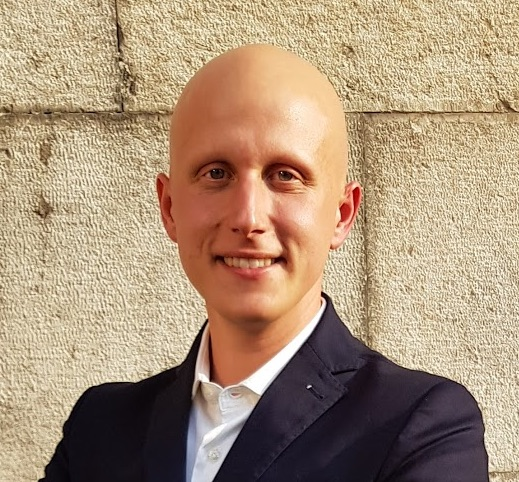
\includegraphics[width=0.8\columnwidth]{matteofico.jpg}\\[\baselineskip] % Your photo
\small % Smaller font size
Matteo Fico \\ % Your name
\url{ficomatteo@gmail.com} \\ % Your email address
\url{linkedin.com/in/matteofico} \\ % Your URL
+39 338 5801268 \\ % Your phone number
\Sep % Some whitespace
I\textbf{ndirizzo:} \\
Via E.Fermi 51 \\ % Address 1
41124, Modena \\ % Address 2
Italia \\ % Address 3
\vfill % Whitespace under this block to push it up under the photo
\end{flushright}
}

%----------------------------------------------------------------------------------------

\begin{document}

\userinformation % Print your information in the left column

\framebreak % End of the first column

%----------------------------------------------------------------------------------------
%	HEADING
%----------------------------------------------------------------------------------------

\cvheading{Matteo Fico} % Large heading - your name

\cvsubheading{Ingegnere Informatico} % Subheading - your occupation/specialization

%----------------------------------------------------------------------------------------
%	ABOUT ME
%----------------------------------------------------------------------------------------

\aboutme{About Me}{
Sono una persona puntuale,  affidabile e a cui piace mettersi in gioco. Ho una grande passione per l'informatica e per le nuove tecnologie. Cerco quotidianamente di migliorarmi sul lavoro e a livello personale. Credo fermamente che con la giusta dose di preparazione e determinazione si possa raggiungere qualsiasi risultato.
	}
\Sep

%----------------------------------------------------------------------------------------
%	EDUCATION
%----------------------------------------------------------------------------------------

\CVSection{Educazione}

%------------------------------------------------

\CVItem{Luglio 2013, Unimore, \textit{Università di Modena e Reggio Emilia}}{Laurea Triennale in Ingegneria Informatica}

%------------------------------------------------

\CVItem{Giugno 2005, ITC Barozzi, \textit{Istituto tecnico commerciale}}{Diploma di perito commerciale, ragioniere e programmatore}

%------------------------------------------------

\Sep % Extra whitespace after the end of a major section

%----------------------------------------------------------------------------------------
%	EXPERIENCE
%----------------------------------------------------------------------------------------

\CVSection{Esperienza}

%------------------------------------------------

\CVItem{Nov 2016 - presente, \textit{R\&D Tecnico di Visione}, Unisorting}{
\begin{itemize}
	\item Lavoro sul campo:
	\begin{itemize}
		\item Testing e raccolta dati presso gli impianti dei clienti
		\item Formazione al cliente sull'utilizzo dei software
		\item Personalizzazioni software 
		\item Demo ( ITA - ENG - ESP )
		\item Supervisione impianto
	\end{itemize}
	\item Lavoro in ufficio:
	\begin{itemize}
		\item Personalizzazione delle impostazioni software
		\item Creazione e testing di nuove features
		\item Supporto tecnico da remoto
		\item Analisi dati e studi di fattibilità sui dati raccolti
		\begin{itemize}
			\item Analisi e organizzazione dati con Python and Excel
		\end{itemize}
	\end{itemize}
		\item Sviluppo software:
		\begin{itemize} 
		\item C\# Sofrware di gestione dati e interfaccia
		\item Python per analisi dei dati e prototipazione rapida
		\end{itemize}
\end{itemize}
}

%------------------------------------------------

\CVItem{Ago 2013 - Nov 2016, \textit{Sviluppo Software}, Datagraph S.r.l.}{Sviluppo e manutenzione software di contabilità pubblica:
\begin{itemize}
	\item Analisi, sviluppo e manutenzione software
	\item Creazione e aggiornamento di query SQL 
	\item Manutenzione MS SQL Server
	\item Assistenza da remoto
\end{itemize}}

\CVItem{Set 2012 - Ago 2013, \textit{Tecnico Software}, Spin S.r.l.}{ 
\begin{itemize}
	\item Tesi di laurea "Interfacciamento di un sistema di pesatura ed etichettatura"
	\item HMI e SCADA per acquisizione e controllo dati.
	\item MS SQL - Creazione e aggiornamento di store-procedure
\end{itemize}}


%----------------------------------------------------------------------------------------
%	NEW PAGE DELIMITER
%	Place this block wherever you would like the content of your CV to go onto the next page
%----------------------------------------------------------------------------------------

\clearpage % Start a new page

\userinformation % Print your information in the left column

\framebreak % End of the first column

\Sep % Extra whitespace after the end of a major section

%----------------------------------------------------------------------------------------
%	IT SKILLS
%----------------------------------------------------------------------------------------

\CVSection{Competenze IT}

%------------------------------------------------

\CVItem{Programmazione}
{C\#, Python}

%------------------------------------------------

\CVItem{DBMS}
{MS SQL, MySQL}

%------------------------------------------------

\CVItem{Web}
{HTML, CSS}

%------------------------------------------------

\CVItem{Source Control}
{Mercurial, GIT, SVN}

%------------------------------------------------

\CVItem{OS}
{Windows, Mac Os X, Unix/Linux}

%----------------------------------------------------------------------------------------
%	PERSONAL SKILLS
%----------------------------------------------------------------------------------------

\Sep % Extra whitespace after the end of a major section

\CVSection{Competenze personali}

\CVItem{Problem-solving and decision-making}{Entrambi migliorati grazie al lavoro sul campo }

\CVItem{Lavoro di squadra}{Migliorato lavorando a progetti complessi e multi disciplinari}

\CVItem{Adattabilità}{Spirito di osservazione e motivazione aiutano ad adattarsi alle varie situazioni lavorative}

\CVItem{Puntualità}{Essere puntuale è una forma di rispetto e di professionalitaà}

\CVItem{Creatività}{Mi piace la grafica, il design e mi appassiona la creazione di interfacce utente}

%------------------------------------------------

\Sep % Extra whitespace after the end of a major section

\CVSection{Lingue}

%------------------------------------------------

\CVItem{Italiano}{Madrelingua} 

\CVItem{Inglese}{Conoscenza professionale}

\CVItem{Spagnolo}{Utilizzo lavorativo tecnico}

\CVItem{Francese}{Elementare}

\Sep

%----------------------------------------------------------------------------------------
%	INTERESTS
%----------------------------------------------------------------------------------------

\CVSection{Interessi}

%------------------------------------------------

\CVItem{Professionali}{Data Analysis, Software Management, UX/UI, Machine Learning}

\CVItem{Personali}{Fotografia, viaggi, musica, cucina, escursionismo}

%------------------------------------------------

\Sep % Extra whitespace after the end of a major section

%----------------------------------------------------------------------------------------


\end{document}


